\chapter{Matrisoperationer}
\paragraph{Definition} En \underline{matris} är ett tvådimensionellt fält av reella tal.
Om matrisen har m rader och n kolumner sägs det vara en $(m\times n)$-matris, eller en matris av typ $m\times n$.
$\begin{pmatrix}
    a_{1,1} & a_{1,2} & \ldots & a_{1,n}\\
    a_{2,1} & a_{2,2} & \vdots & \\
    \ldots
\end{pmatrix}$
Matriser av samma typ adderas komponentvis. Exempelvis:\\
$\begin{pmatrix}
    1&2\\4&3
\end{pmatrix}+\begin{pmatrix}
    5&8\\6&7
\end{pmatrix}=
\begin{pmatrix}
    1+5&2+8\\4+6&3+7
\end{pmatrix}=\begin{pmatrix}
    6&10\\10&10
\end{pmatrix}$
Matriser av olika typ adderas inte!
Vi har sett exempel på matriser i kolonnvektorer.
En matris på formen $\begin{pmatrix}a_{1}&a_{2}&\hdots&a_{n}\end{pmatrix}$ är en radvektor.

Produkten av en matris med ett reellt tal definieras också "komponentvis". Exempelvis:\\
$2\cdot \begin{pmatrix}
    2&6\\4&8
\end{pmatrix}=\begin{pmatrix}
    3\cdot 2&3\cdot 6\\3\cdot 4&3\cdot 8
\end{pmatrix}=\begin{pmatrix}
    6&18\\12&24
\end{pmatrix}$

\paragraph{Definition} Givet en $3\times 3$-matris $A=\begin{pmatrix}
    \line(0,1){8}&\line(0,1){8}&\line(0,1){8}\\
    a_{1}&a_{2}&a_{3}\\
    \line(0,1){8}&\line(0,1){8}&\line(0,1){8}
\end{pmatrix}$ och en (kolumn)vektor $\bm{v}=\begin{pmatrix}v_{1}\\v_{2}\\v_{3}\end{pmatrix}$ definierar vi deras
produkt som  % fyll i

\paragraph{Proposition 2.11} 
\begin{enumerate}
    \item $A+B=B+A$
    \item $A(\bm{u}+\bm{v})=$
    \item $(A+B)\bm{v}=A\bm{v}+B\bm{v}$
    \item $A(c\bm{v})=c(A\bm{v})=(cA)\bm{v}$
\end{enumerate}
\section{Produkter av matriser}
\paragraph{Definition} Låt A och B vara $3\times 3$-matriser och $B=\begin{pmatrix}
    \line(0,1){8}&\line(0,1){8}&\line(0,1){8}\\
    \bm{b}_{1}&\bm{b}_{2}&\bm{b}_{3}\\
    \line(0,1){8}&\line(0,1){8}&\line(0,1){8}
\end{pmatrix}$.\\
Vi definierar produkten av A och B genom $AB=A\begin{pmatrix}
    \line(0,1){8}&\line(0,1){8}&\line(0,1){8}\\
    \bm{b}_{1}&\bm{b}_{2}&\bm{b}_{3}\\
    \line(0,1){8}&\line(0,1){8}&\line(0,1){8}
\end{pmatrix}=\begin{pmatrix}
    \line(0,1){8}&\line(0,1){8}&\line(0,1){8}\\
    A\bm{b}_{1}&A\bm{b}_{2}&A\bm{b}_{3}\\
    \line(0,1){8}&\line(0,1){8}&\line(0,1){8}
\end{pmatrix}$

\paragraph{Ex} Låt $A=\begin{pmatrix}0&2\\4&6\end{pmatrix}$ och $B=\begin{pmatrix}1&3\\5&7\end{pmatrix}$.
Beräkna AB och BA.
\subparagraph{Lösning} 
$AB=\begin{pmatrix}
    0&2\\4&6
\end{pmatrix}
\begin{pmatrix}
    1&3\\5&7
\end{pmatrix}=
\begin{pmatrix}
    10&14\\34&54
\end{pmatrix}$
% Fyll i resten av lösningen \\

\paragraph{Proposition 2.14} Låt A  och B vara $n\times n$-matriser där A på position $(i,j)$ har talet $a_{ij}$ och B på position $(i,j)$ har talet $b_{ij}$.
Låt $C=AB$ och låt $c_{ij}$ vara talet för C på position $(i,j)$.
Då $c_{ij}=\sum^{n}_{k=1}a_{ik}b_{kj}$.\\
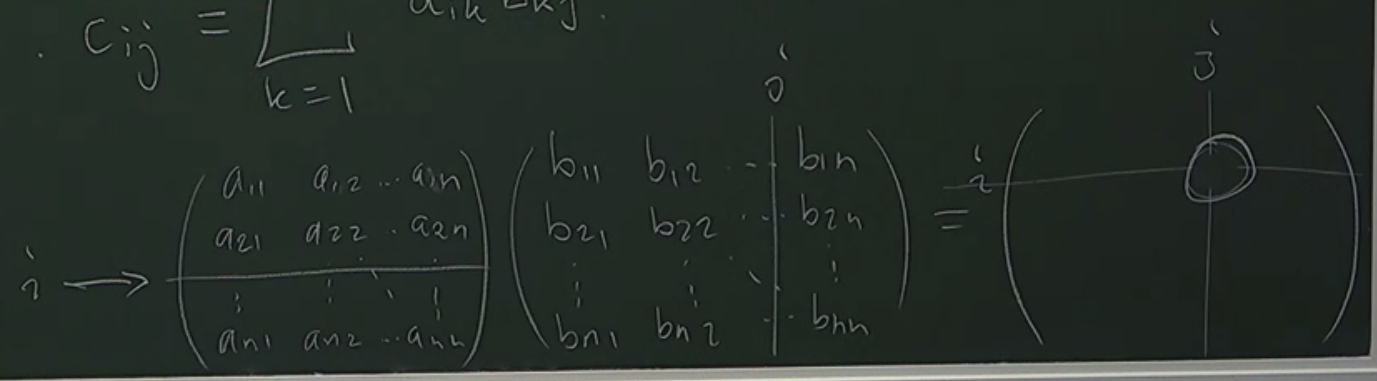
\includegraphics[scale=0.3]{imgs/22-01-31-img01.png}\\
Låt oss använda Prop 2.14 för att beräkna AB från exemplet ovan:\\
%fyll i missat
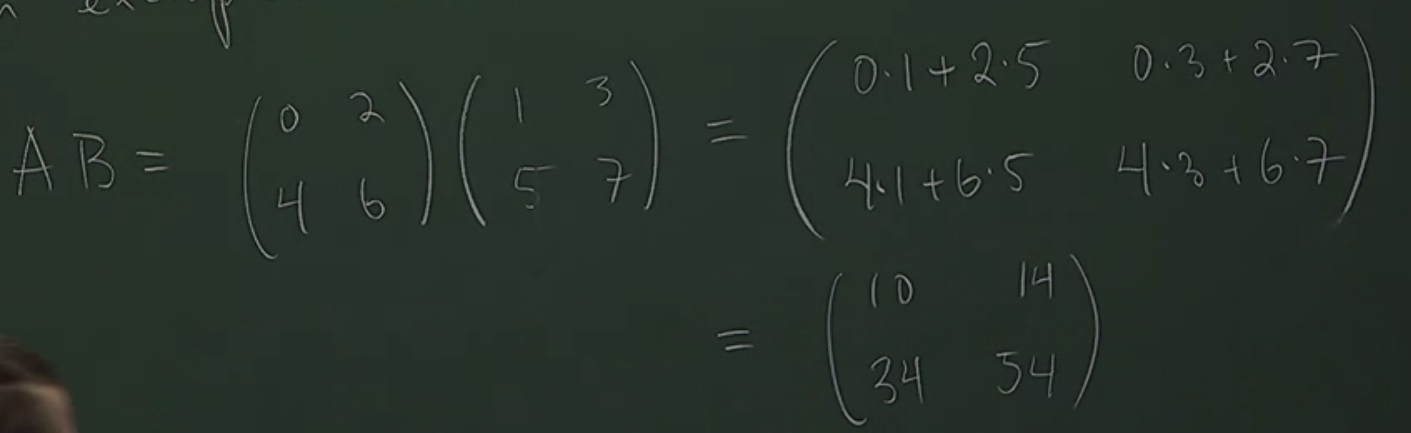
\includegraphics[scale=0.3]{imgs/22-01-31-img02.png}\\
\paragraph{Propostion 2.16} Låt $A,B,C$ vara $n\times n$-matriser.
\begin{enumerate}
    \item $A(cB)=c(AB)=(cA)B$
    \item $A(B+C)=AB+AC$
    \item $(B+C)A=BA+CA$
    \item $A(B\bm{v})=(AB)\bm{v}$
    \item $A(BC)=(AB)C$
\end{enumerate}
Kom ihåg att $AB\neq BA$!

\paragraph{Definition} Givet en $m\times n$-matris A så ges dess \underline{transponat},$A^{t}$, av den $n\times m$-matris av att $a^{t}_{ij}=a_{ji}$.

\paragraph{Ex} Om $a=\begin{pmatrix}
    1&2&4\\3&6&9
\end{pmatrix}$ då $A^{t}=\begin{pmatrix}
    1&3\\2&6\\4&9
\end{pmatrix}$

\paragraph{Definition} En $n\times n$-matris A sägs vara \underline{symmetrisk} om $A^{t}=A$.

\paragraph{Ex} Matriserna $\begin{pmatrix}1&5\\5&3\end{pmatrix}$ och $\begin{pmatrix}1&0&-1\\0&2&10\\-1&10&8\end{pmatrix}$ är symmetriska.

\paragraph{Proposition 2.21} Låt A,B vara $n\times n$-matriser.
\begin{enumerate}
    \item $(a^{t})^{t}=A$
    \item $(A+B)^{t}=A^{t}+B^{t}$
    \item $(cA)^{t}=cA^{t}$
    \item $(AB)^{t}=B^{t}A^{t}$
\end{enumerate}

\chapter{Determinanter (Avs. 2.2)}
\paragraph{Definition} Givet en $2\times 2$-matris $a=\begin{pmatrix}a&b\\c&d\end{pmatrix}$ låter vi dess \underline{determinant} vara $det(A)=\begin{vmatrix}a&b\\c&d\end{vmatrix}=ad-bc$.

\paragraph{Ex} Om $A=\begin{pmatrix}
    2&0\\0&1
\end{pmatrix}$ då är $det(A)=\begin{vmatrix}
    2&0\\0&1
\end{vmatrix}=2\cdot 1-0\cdot 0=2$.
Om vi låter $\bm{u}=\begin{pmatrix}
    2\\0
\end{pmatrix}$, $\bm{v}=\begin{pmatrix}
    0\\1
\end{pmatrix}$ då är arean av parallellogramet som $\bm{u}$ och $\bm{v}$ spänner 2.\\
%\includegraphics[scale=0.3]{imgs/22-01-31-img03.png}\\

\paragraph{Sats 2.24} Låt $A=\begin{pmatrix}\bm{u}&\bm{v}\end{pmatrix}=\begin{pmatrix}a&b\\c&d\end{pmatrix}$och låte D vara parallellogramet som spänns av $\bm{u}$ och $\bm{v}$.
Då är $|det(A)|=area(D)$.
Dessutom är $det(A)>0$ om och endast om vinkeln mellan $\bm{u}$ och $\bm{v}$, då $\bm{u}$ vrids moturs till $\bm{v}$, är mellan 0 och $\pi$.\\
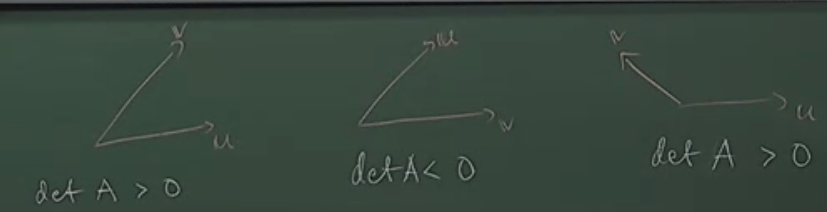
\includegraphics[scale=0.5]{imgs/22-01-31-img04.png}
\subparagraph{Bevis} Vad är $area(D)$?
Låt L vara en linje som är ortogonal mot $\bm{u}=\begin{pmatrix}
    a\\c
\end{pmatrix}$.
Då är $\bm{r}=\begin{pmatrix}
    c\\-a
\end{pmatrix}$ en riktningsvektor för L ty $\bm{r}\cdot \bm{u}=0$.\\
$area(D)=
||\bm{u}||\cdot ||\bm{v}_{L}||=
||\bm{u}||\cdot ||\frac{\bm{v}\cdot \bm{r}}{\bm{r}\cdot \bm{r}}||
=||\bm{u}||\cdot \frac{|\bm{v}\cdot \bm{r}}{||\bm{r}^{2}||}\cdot ||\bm{r}||=
\frac{||\bm{u}||}{||\bm{r}||}|\bm{v}\cdot\bm{r}=
\frac{\sqrt{a^{2}+c^{2}}}{\sqrt{c^{2}+(-a)^{2}}}|\begin{pmatrix}
    b\\d
\end{pmatrix}\cdot \begin{pmatrix}c\\-a\end{pmatrix}|=
bc-da|=
|ad-bc=
|det(A)|$

Observera att Sats 2.24 speciellt ger att $det(A)=0\Leftrightarrow \bm{u},\bm{v}$ parallella

\paragraph{Definition} Låt $A=\begin{pmatrix}
    x_{1} & x_{2} & x_{3}\\
    y_{1} & y_{2} & y_{3}\\
    z_{1} & z_{2} & z_{3}\\
\end{pmatrix}$.
Då ges dess determinant av $det(A)=\begin{vmatrix}
    x_{1} & x_{2} & x_{3}\\
    y_{1} & y_{2} & y_{3}\\
    z_{1} & z_{2} & z_{3}\\
\end{vmatrix}=x_{1}(y_{2}z_{3}-z_{2}y_{3})-x_{2}(y_{1}z_{3}-z_{1}y_{3})+x_{3}(y_{1}z_{2}-z_{1}y_{2})$

En minnesregel för kryssprodukt:\\
$\bm{u}=\begin{pmatrix}
    u_{1}\\u_{2}\\u_{3}
\end{pmatrix},
\bm{v}=\begin{pmatrix}
    v_{1}\\v_{2}\\v_{3}
\end{pmatrix}$
i $e_{x},e_{y},e_{z}$.
Då ges $\bm{u}\times \bm{v}=\begin{vmatrix}
    e_{x}&e_{y}&e_{z}\\
    u_{1}&u_{2}&u_{3}\\
    v_{1}&v_{2}&v_{3}
\end{vmatrix}=e_{x}(u_{2}v_{3}-v_{2}u_{3})-e_{y}(u_{1}v_{3}-v_{1}u_{3})+e_{z}(u_{1}v_{2}-v_{1}u_{2})$